\section{Questo esperimento come metodo didattico}
\todo{posso lasciare questo?}
Qui dovrei inserire una foto della notte dei ricercatori. Non ho foto di quella sera,
quindi metto una foto del mio gatto al suo posto.

\begin{figure}[H]
    \centering
    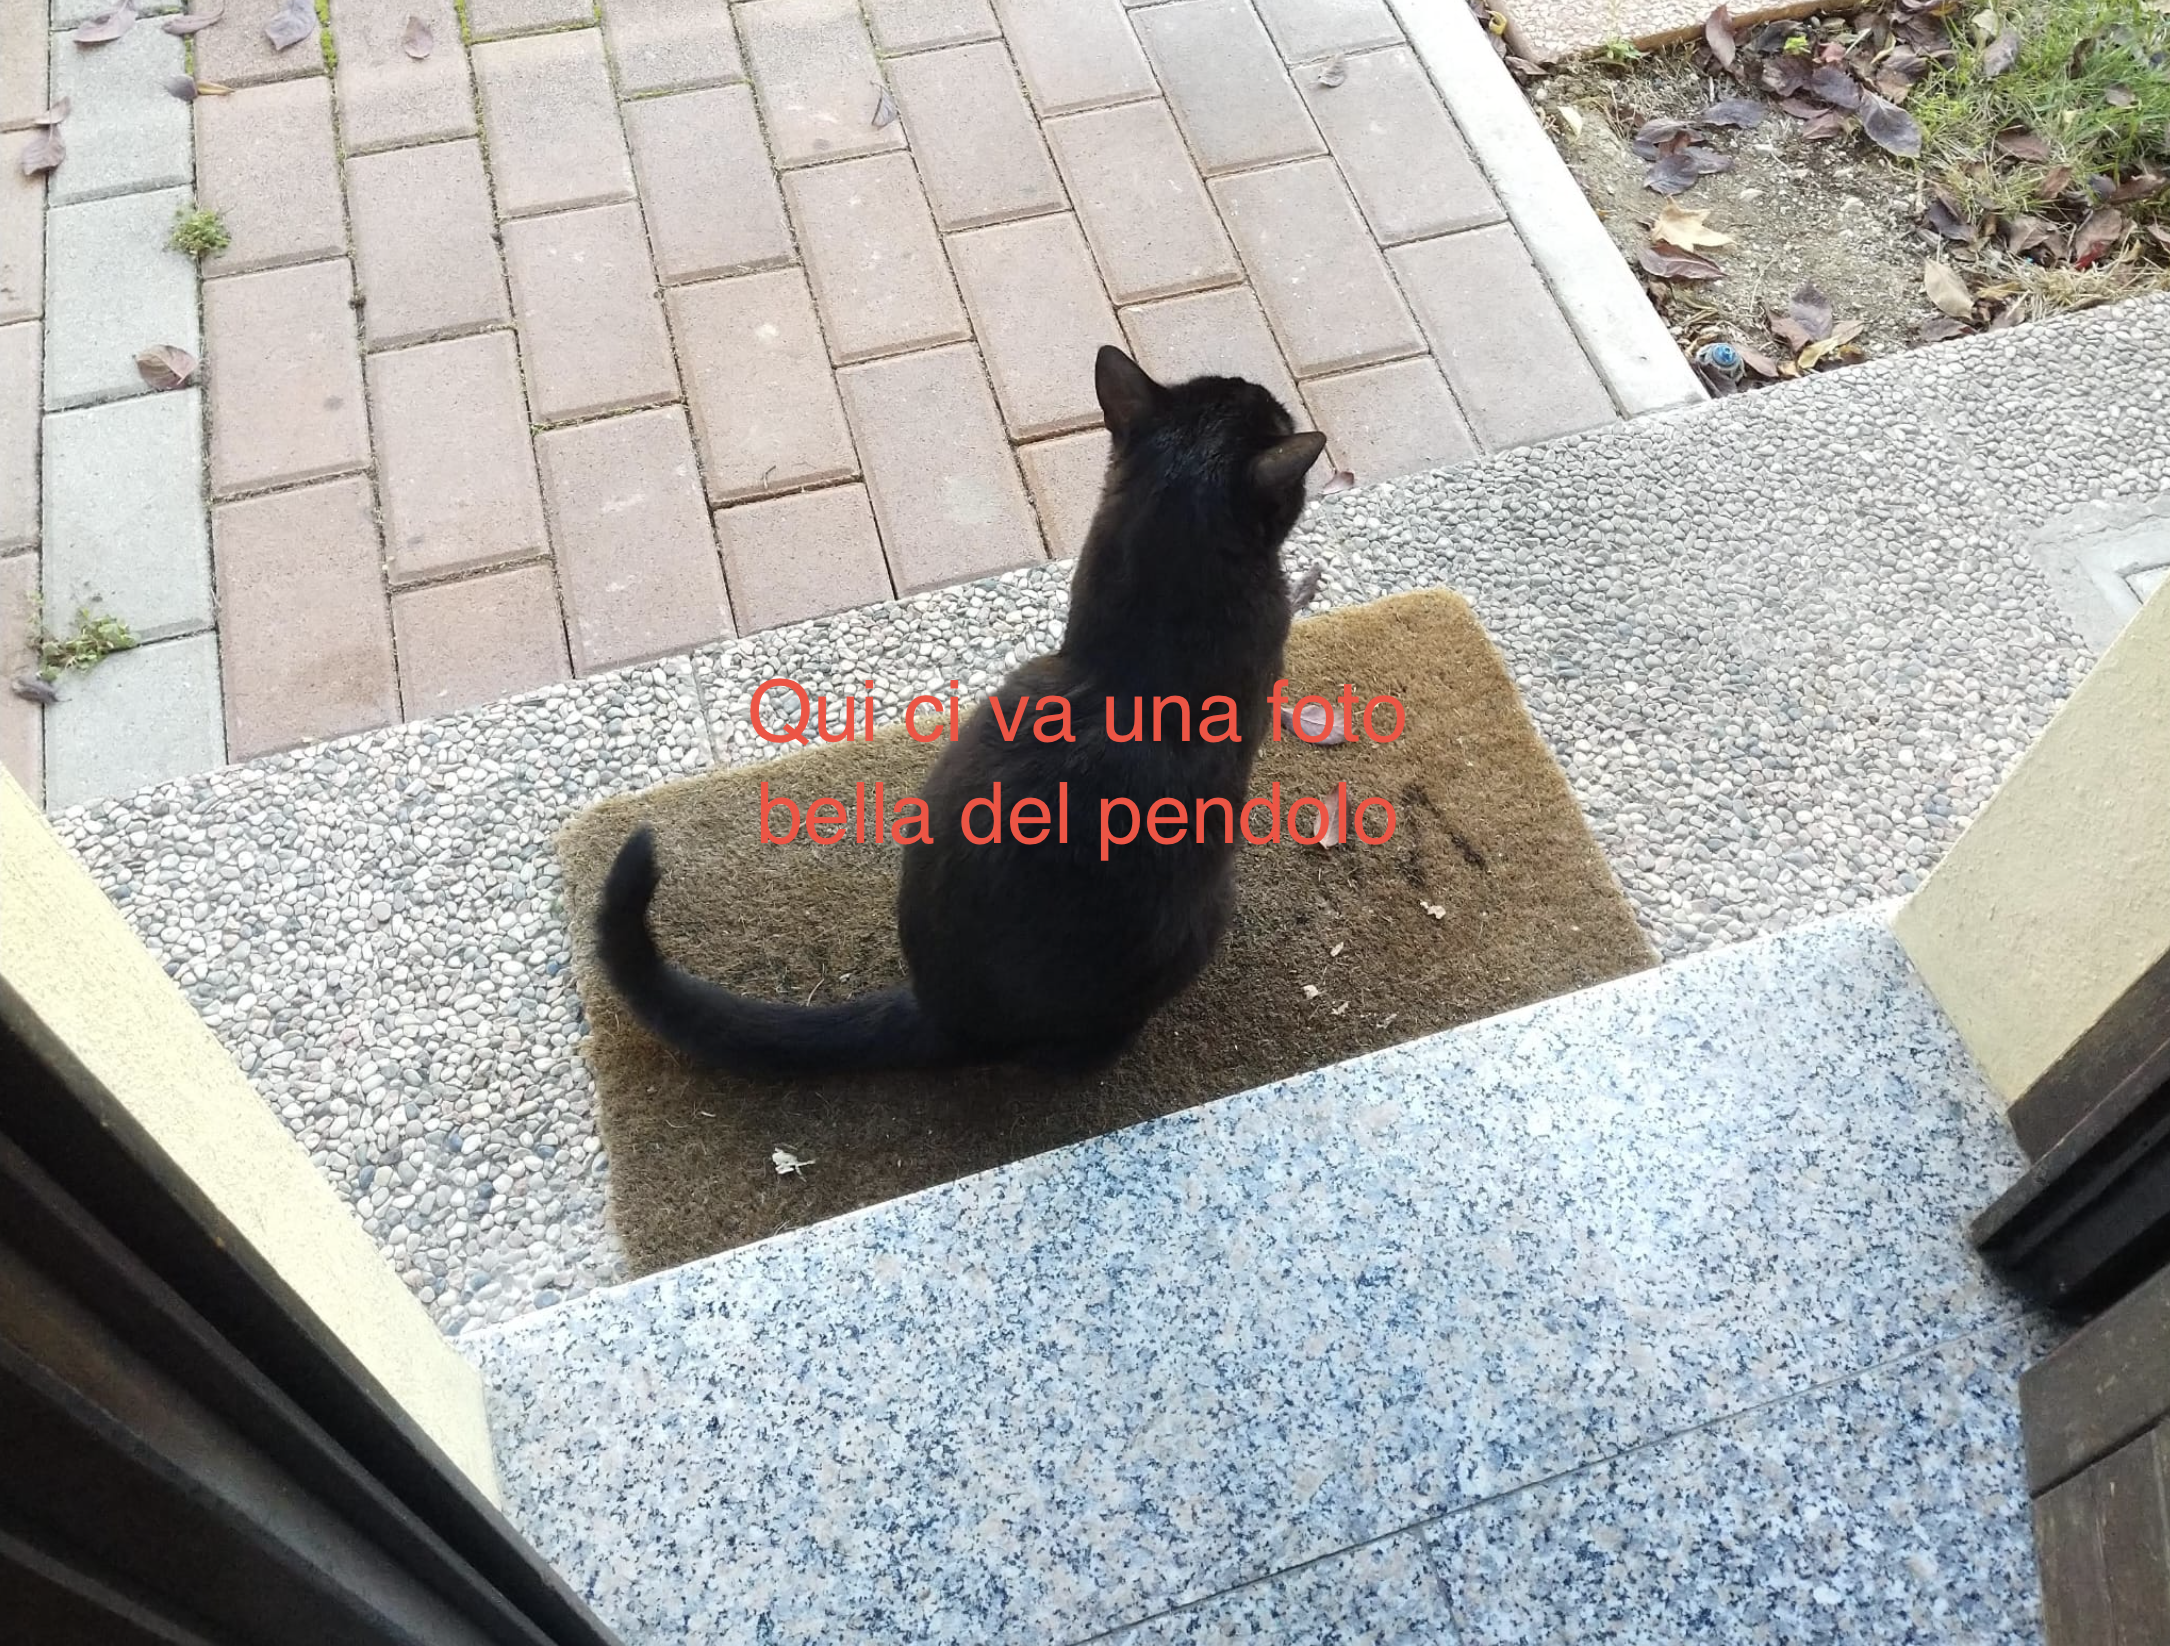
\includegraphics[width=\textwidth]{docs/report/assets/foto-pendolo.png}
    \caption[Noir]{
        Il mio gatto, Noir. Il gatto è seduto davanti alla porta di
        casa mia, perso nell'atto di contemplare il sole di una fresca domenica mattina di
        ottobre. Il gatto non influenza, ne' è influenzato in alcun modo dalla ricerca svolta in questa tesi (o da qualsiasi ricerca scientifica in generale).
        I gatti sono animali particolari, in quanto non possono essere considerati
        addomesticabili nello stesso modo di altri animali da compagnia. In un certo
        senso, si potrebbe dire che il gatto è un sistema non controllabile.
    }
    \label{fig:noir}
\end{figure}
